\documentclass[a4paper]{article}
\usepackage[affil-it]{authblk}
\usepackage[backend=bibtex,style=numeric]{biblatex}
\usepackage{graphicx}
\usepackage{amsmath}
\usepackage{geometry}
\usepackage{array}
\usepackage{caption}
\usepackage{subcaption}
\usepackage{tcolorbox}
\usepackage{booktabs}
\usepackage{caption}
\geometry{margin=1.5cm, vmargin={0pt,1cm}}
\setlength{\topmargin}{-1cm}
\setlength{\paperheight}{29.7cm}
\setlength{\textheight}{25.3cm}

\begin{document}

% =================================================
\title{Project Report}

\author{Yuwei Liang 3230102923
  \thanks{Electronic address: \texttt{liangyuwei631@gmail.com}}}
\affil{(Mathematics and Applied Mathematics 2302), Zhejiang University}

\date{\today}

\maketitle

\begin{abstract}
  This report presents the results of the project, which involves the implementation and evaluation of various interpolation and curve fitting techniques. The project includes the interpolation of the Runge function using natural cubic splines, B-splines, and curve fitting using B-splines. The results demonstrate the effectiveness of these techniques in approximating functions and curves. Additionally, the report includes a test to confirm the equivalence of the PPform and Bform representations of cubic splines. Finally, the implementation and evaluation of arbitrary degree B-splines are discussed, demonstrating the correctness of the implementation.
\end{abstract}

% ============================================

\section*{A. RungeFunction}
First, I interpolate Runge function with natural cubic spline with N = 6, 11, 21, 41, 51, the result is shown in Figure \ref{fig:runge_interpolation} and the error is shown in table\ref{tab:max_error}.
We can see that for cubic-spline interpolation, the Runge phenomenon no longer exists and when N is greater than 11, the interpolated curve almost coincides with the original curve. As N increases, the Max Error decreases significantly.
\begin{figure}[h]
  \centering
  \begin{minipage}{0.6\textwidth} % 左侧图片
    \centering
    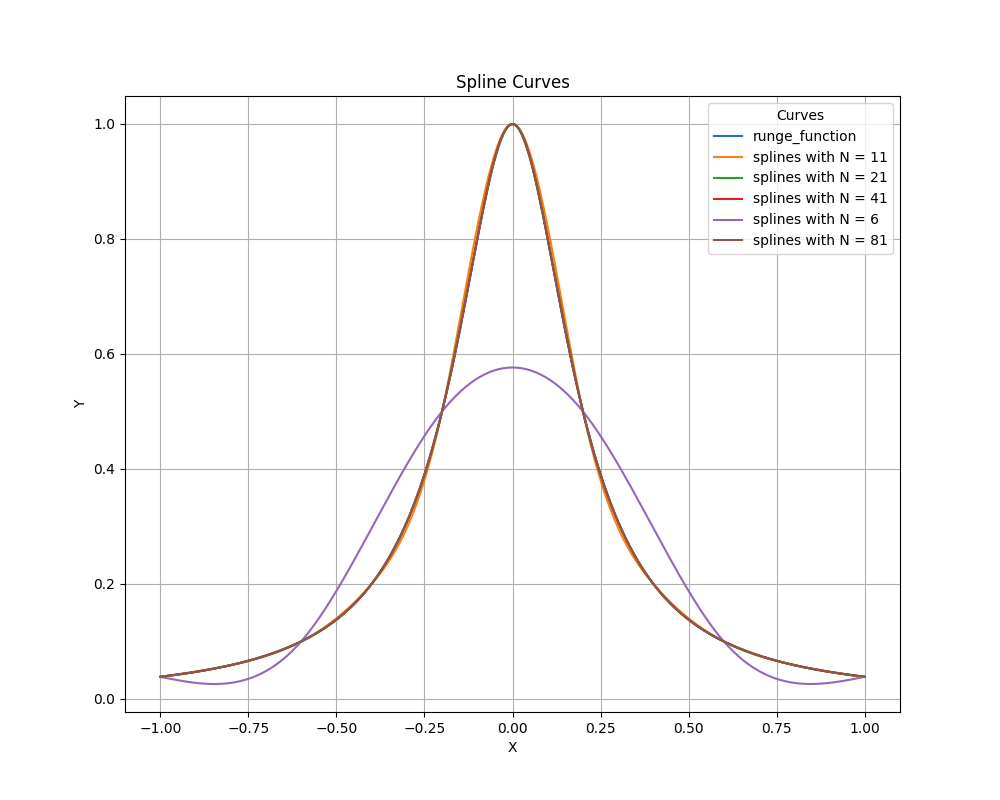
\includegraphics[width=\linewidth]{figures/A.png}
    \caption{Interpolation of Runge function with natural cubic spline}
    \label{fig:runge_interpolation}
  \end{minipage}
  \hfill 
  \begin{minipage}{0.35\textwidth} % 右侧表格
    \centering
    \renewcommand{\arraystretch}{1.2} % 调整表格行间距
    \begin{tabular}{|c|c|}
      \hline
      \textbf{N} & \textbf{Max Error} \\ \hline
      6  & 0.423482    \\ \hline
      11 & 0.0205306   \\ \hline
      21 & 0.00316894  \\ \hline
      41 & 0.000275356 \\ \hline
      81 & 1.609e-05   \\ \hline
    \end{tabular}
    \captionof{table}{Max error for different $N$ values}
    \label{tab:max_error}
  \end{minipage}
\end{figure}

\newpage

\section*{C\&D. BSpline}

The result of B-Spline interpolation is shown in Figure \ref{fig:bspline_interpolation} and the error at specific nodes is shown is table \ref{tab:interpolation_errors}. We can see that cubic complte BSpline interpolation has a better performance than quartic bspline interpolation.

The machchine precision is due to the floating point error, which is inevitable in the numerical computation.

\begin{figure}[h]
  \centering
  \begin{minipage}{0.6\textwidth} % 左侧图片
    \centering
    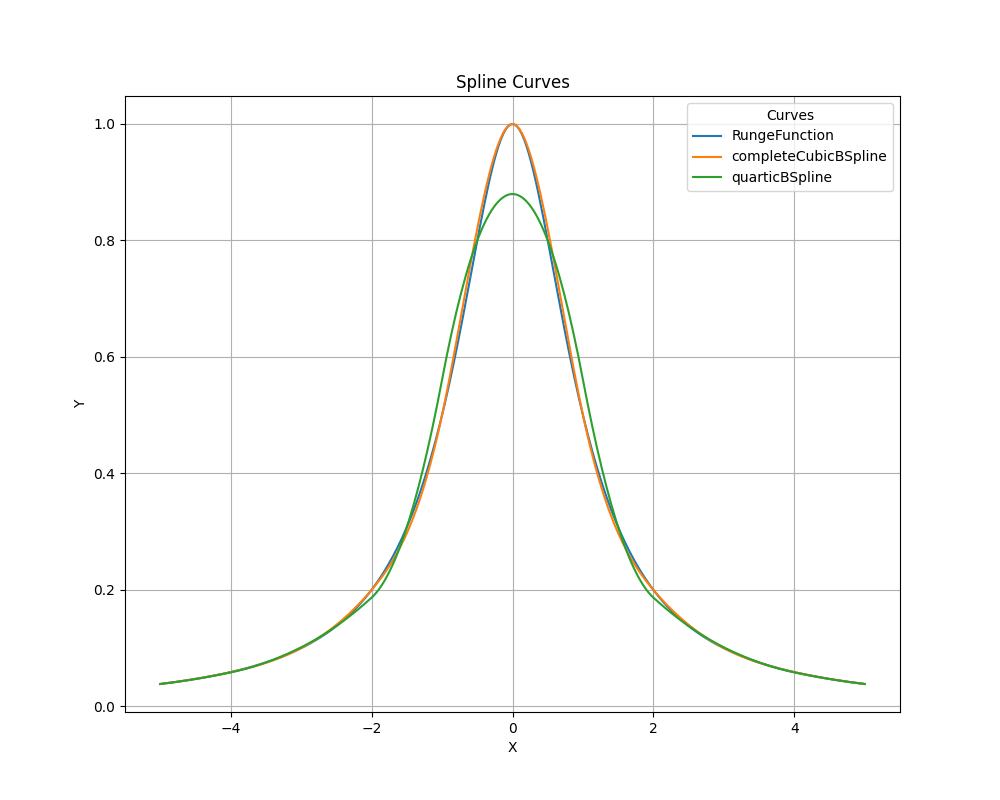
\includegraphics[width=\linewidth]{figures/C.png}
    \caption{Interpolation of Runge function with B-Spline}
    \label{fig:bspline_interpolation}
  \end{minipage}
  \hfill
  \begin{minipage}{0.35\textwidth} % 右侧表格
    \centering
    \renewcommand{\arraystretch}{1.2} % 调整表格行间距
    \begin{tabular}{|c|c|c|}
      \hline
      \textbf{x} & \textbf{Cubic Error} & \textbf{Quartic Error} \\ \hline
      -3.5       & 0.000669568                    & 0                                \\ \hline
      -3         & 0                              & 0.00141838                       \\ \hline
      -0.5       & 0.0205289                      & 1.11022e-16                      \\ \hline
       0         & 0                              & 0.120238                         \\ \hline
       0.5       & 0.0205289                      & 1.11022e-16                      \\ \hline
       3         & 1.38778e-17                    & 0.00141838                       \\ \hline
       3.5       & 0.000669568                    & 1.38778e-17                      \\ \hline
    \end{tabular}
    \captionof{table}{Interpolation errors for different B-Spline types}
    \label{tab:interpolation_errors}
  \end{minipage}
\end{figure}

\newpage

\section*{E. Curve Fitting}

The result of the curve fitting is shown in Figure \ref{fig:curve_fitting}. The second and fourth columns are the fittings with equidistant nodes. The number after "curve\_fitting" in the caption indicates the number of control points. It can be seen that as $N$ increases, the fitting effect of the curve improves. Overall, the effect of equidistant nodes is better than the other type. However, for the second figure, due to the equidistant drawing, it loses the details of the innermost circle.

\begin{figure}[htbp]
  \centering
  % Row 1
  \begin{subfigure}[t]{0.24\textwidth}
      \centering
      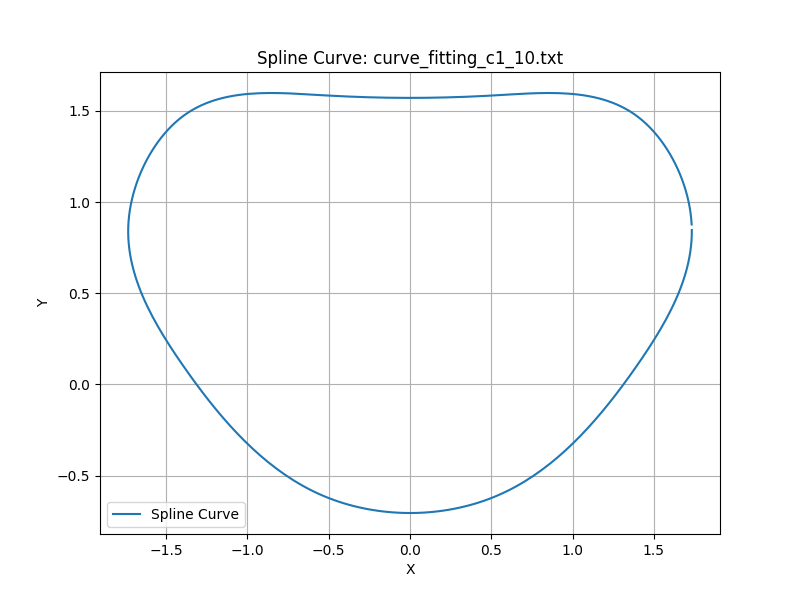
\includegraphics[width=\textwidth]{figures/E/curve_fitting_c1_10.png}
      \caption*{curve\_fitting\_c1\_10}
  \end{subfigure}
  \begin{subfigure}[t]{0.24\textwidth}
      \centering
      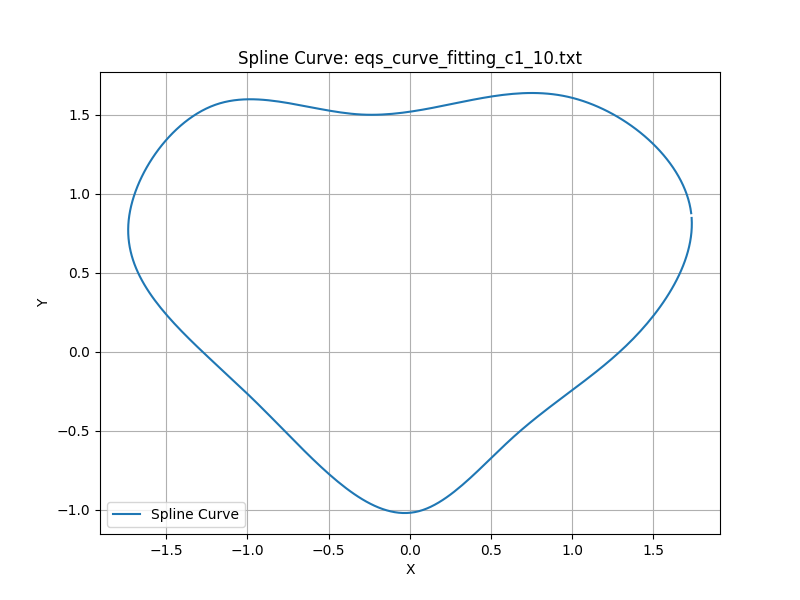
\includegraphics[width=\textwidth]{figures/E/eqs_curve_fitting_c1_10.png}
      \caption*{eqs\_curve\_fitting\_c1\_10}
  \end{subfigure}
  \begin{subfigure}[t]{0.24\textwidth}
      \centering
      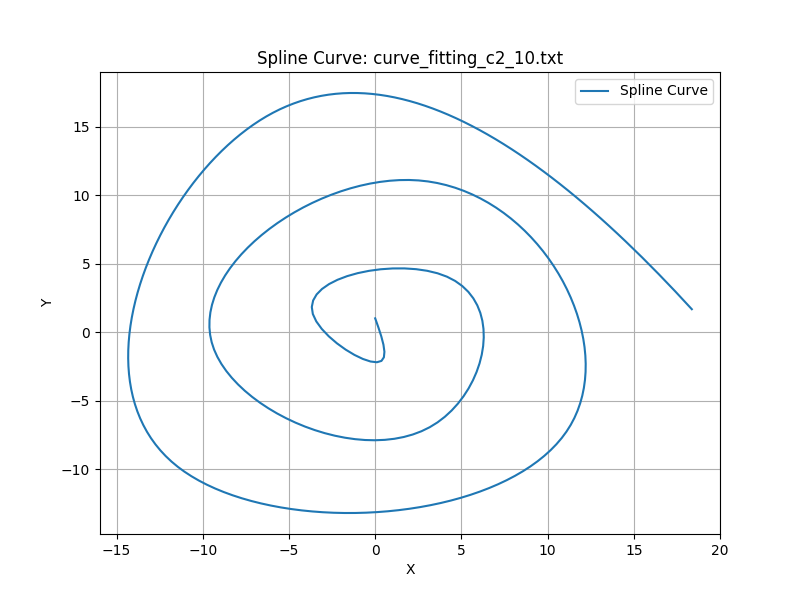
\includegraphics[width=\textwidth]{figures/E/curve_fitting_c2_10.png}
      \caption*{curve\_fitting\_c2\_10}
  \end{subfigure}
  \begin{subfigure}[t]{0.24\textwidth}
      \centering
      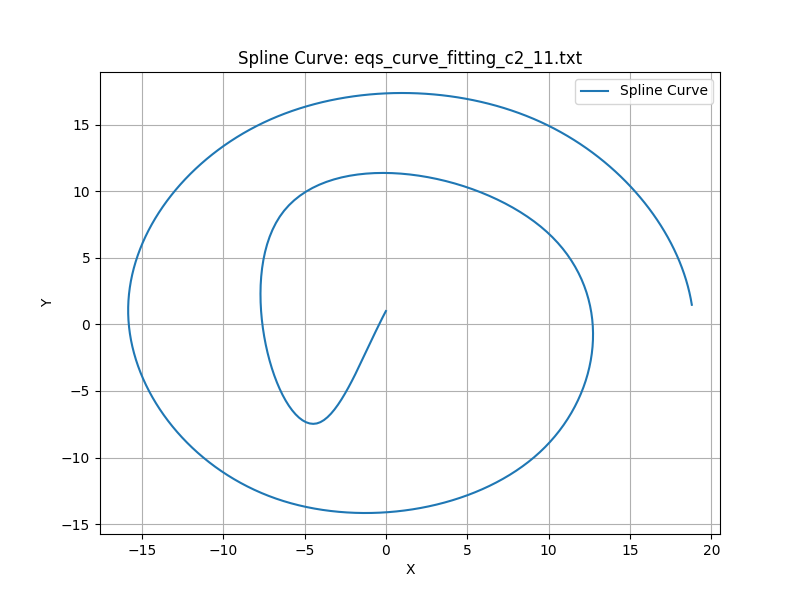
\includegraphics[width=\textwidth]{figures/E/eqs_curve_fitting_c2_11.png}
      \caption*{eqs\_curve\_fitting\_c2\_11}
  \end{subfigure}

  % Row 2
  \begin{subfigure}[t]{0.24\textwidth}
      \centering
      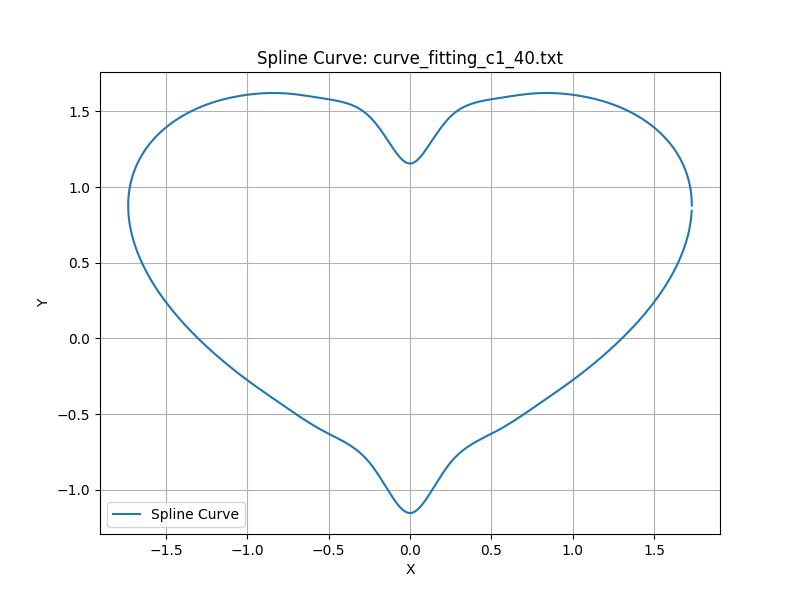
\includegraphics[width=\textwidth]{figures/E/curve_fitting_c1_40.png}
      \caption*{curve\_fitting\_c1\_40}
  \end{subfigure}
  \begin{subfigure}[t]{0.24\textwidth}
      \centering
      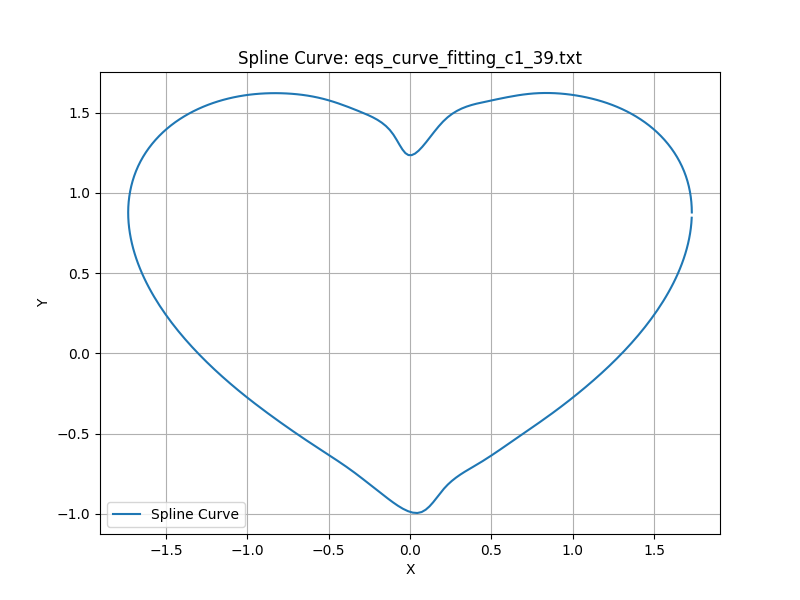
\includegraphics[width=\textwidth]{figures/E/eqs_curve_fitting_c1_39.png}
      \caption*{eqs\_curve\_fitting\_c1\_39}
  \end{subfigure}
  \begin{subfigure}[t]{0.24\textwidth}
      \centering
      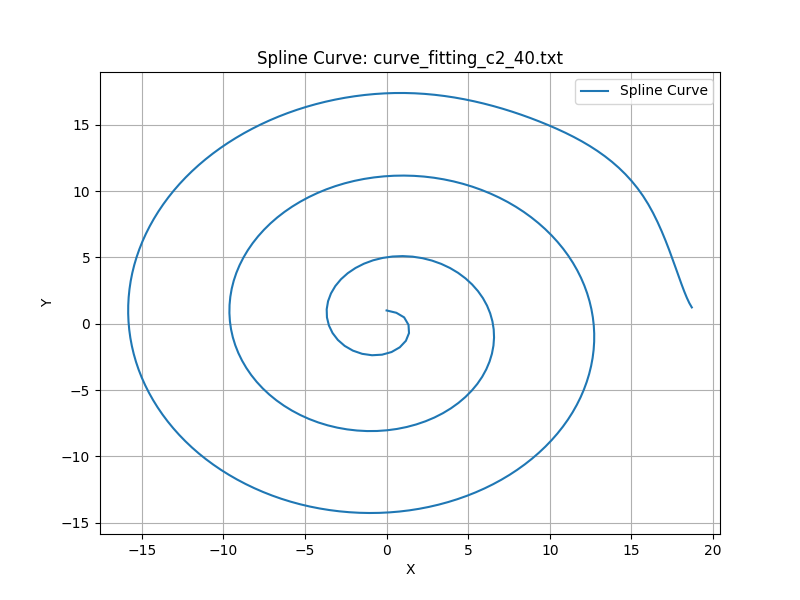
\includegraphics[width=\textwidth]{figures/E/curve_fitting_c2_40.png}
      \caption*{curve\_fitting\_c2\_40}
  \end{subfigure}
  \begin{subfigure}[t]{0.24\textwidth}
      \centering
      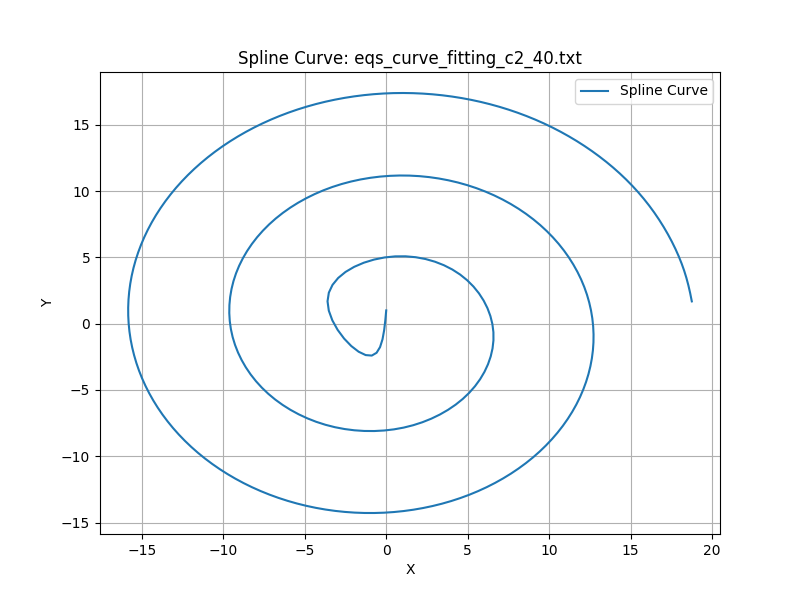
\includegraphics[width=\textwidth]{figures/E/eqs_curve_fitting_c2_40.png}
      \caption*{eqs\_curve\_fitting\_c2\_40}
  \end{subfigure}

  % Row 3
  \begin{subfigure}[t]{0.24\textwidth}
      \centering
      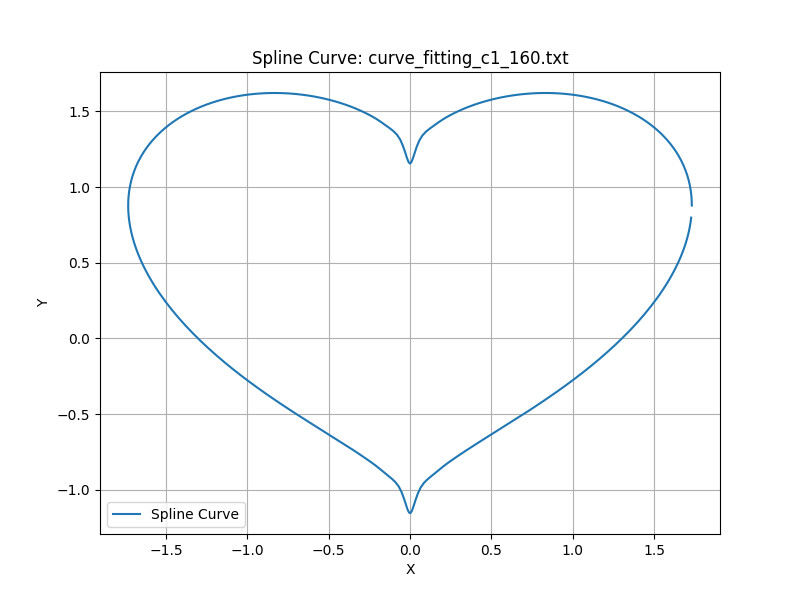
\includegraphics[width=\textwidth]{figures/E/curve_fitting_c1_160.png}
      \caption*{curve\_fitting\_c1\_160}
  \end{subfigure}
  \begin{subfigure}[t]{0.24\textwidth}
      \centering
      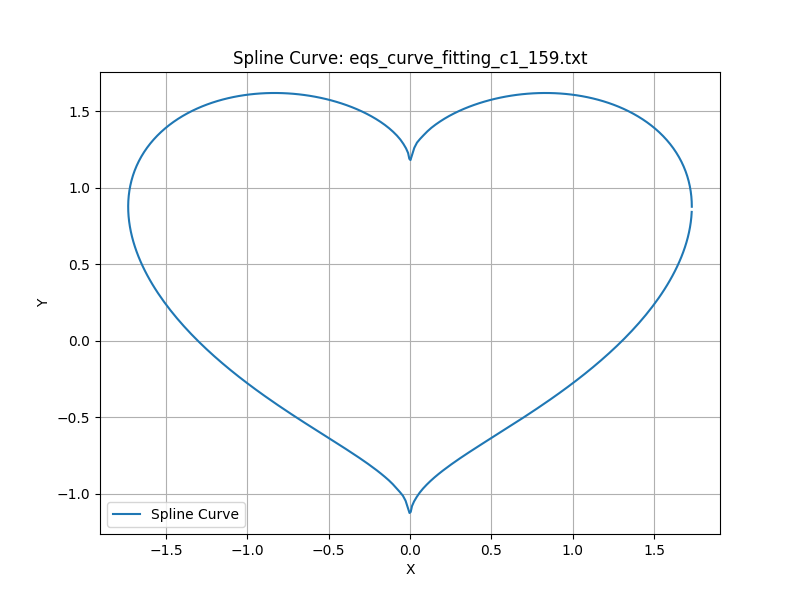
\includegraphics[width=\textwidth]{figures/E/eqs_curve_fitting_c1_159.png}
      \caption*{eqs\_curve\_fitting\_c1\_159}
  \end{subfigure}
  \begin{subfigure}[t]{0.24\textwidth}
      \centering
      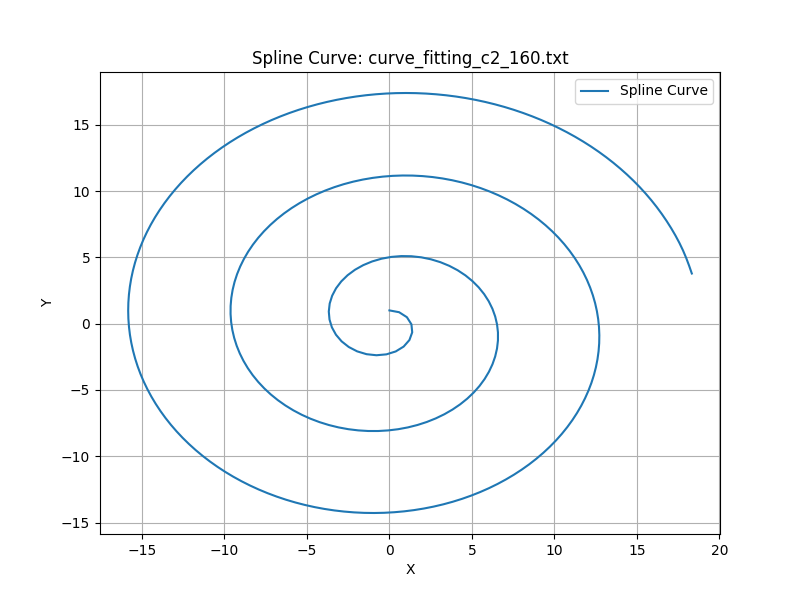
\includegraphics[width=\textwidth]{figures/E/curve_fitting_c2_160.png}
      \caption*{curve\_fitting\_c2\_160}
  \end{subfigure}
  \begin{subfigure}[t]{0.24\textwidth}
      \centering
      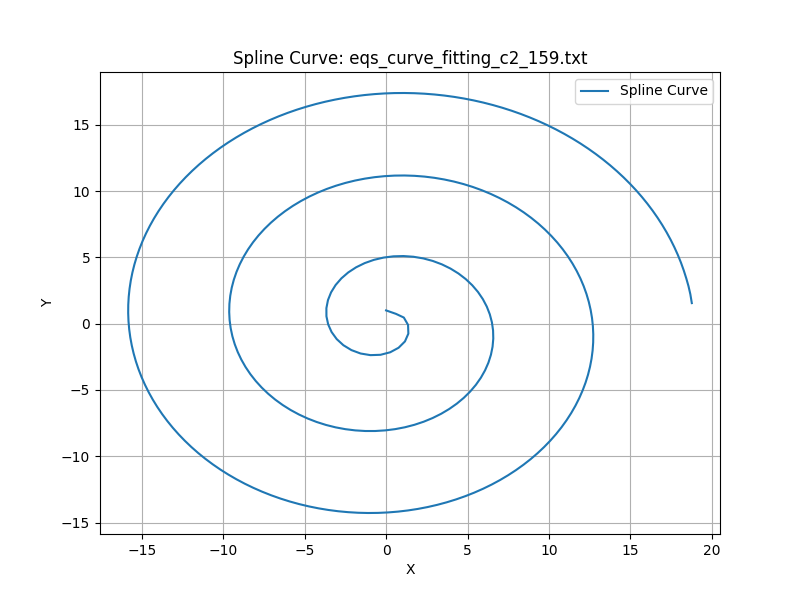
\includegraphics[width=\textwidth]{figures/E/eqs_curve_fitting_c2_159.png}
      \caption*{eqs\_curve\_fitting\_c2\_159}
  \end{subfigure}
  \caption{Curve fitting with different $N$ values}
  \label{fig:curve_fitting}
\end{figure}

\newpage
\section*{Test: PPform and Bform Have the Same Result}

In this section, we analyze and confirm that the PPform (piecewise polynomial) and Bform (B-spline) representations of cubic splines yield the same results when evaluated at identical points. The test involves three types of cubic splines: Natural, Periodic, and Complete. Two sets of nodes and values are used to validate the results.

\subsection*{Test Setup}

  - First dataset:
    \begin{itemize}
      \item Nodes: $\{1, 2, 4, 5, 7\}$
      \item Values: $\{6, 7, 6, 5, 6\}$
    \end{itemize}
  - Second dataset (based on a function):
    \begin{itemize}
      \item Nodes: $\{-5, -4, -3, -1, 0, 1, 3, 4, 5\}$
      \item Function: $f(x) = \frac{1}{1 + x^2}$
    \end{itemize}

\subsection*{Results for the First Dataset}

The first dataset tests the splines using specified nodes and values. Results are shown below:

\begin{table}[ht]
\centering
\begin{tabular}{|c|c|c|c|c|c|c|}
\hline
$x$ & $N_B$ & $N_{PP}$ & $P_B$ & $P_{PP}$ & $C_B$ & $C_{PP}$ \\
\hline
1.0 & 6.00000 & 6.00000 & 6.00000 & 6.00000 & 6.00000 & 6.00000 \\
1.6 & 6.68981 & 6.68981 & 6.67886 & 6.67886 & 6.80129 & 6.80129 \\
2.2 & 7.07913 & 7.07913 & 7.08309 & 7.08309 & 7.03558 & 7.03558 \\
2.8 & 7.02426 & 7.02426 & 7.03063 & 7.03063 & 6.93910 & 6.93910 \\
3.4 & 6.62448 & 6.62448 & 6.62640 & 6.62640 & 6.57706 & 6.57706 \\
4.0 & 6.00000 & 6.00000 & 6.00000 & 6.00000 & 6.00000 & 6.00000 \\
4.6 & 5.31716 & 5.31716 & 5.32114 & 5.32114 & 5.32374 & 5.32374 \\
5.2 & 4.92348 & 4.92348 & 4.91691 & 4.91691 & 4.92160 & 4.92160 \\
5.8 & 5.00361 & 5.00361 & 4.96937 & 4.96937 & 5.00284 & 5.00284 \\
\hline
\end{tabular}
\caption*{Comparison of spline evaluations for the first dataset.}
\end{table}

\subsection*{Results for the Second Dataset}

The second dataset evaluates the splines based on the function $f(x) = \frac{1}{1 + x^2}$. Results are shown below:

\begin{table}[ht]
\centering
\begin{tabular}{|c|c|c|c|c|c|c|}
\hline
$x$ & $N_B$ & $N_{PP}$ & $P_B$ & $P_{PP}$ & $C_B$ & $C_{PP}$ \\
\hline
-5.0 & 0.03846 & 0.03846 & 0.03846 & 0.03846 & 0.03846 & 0.03846 \\
-3.8 & 0.06667 & 0.06667 & 0.06716 & 0.06716 & 0.06659 & 0.06659 \\
-2.6 & 0.11126 & 0.11126 & 0.11094 & 0.11094 & 0.11131 & 0.11131 \\
-1.4 & 0.30802 & 0.30802 & 0.30790 & 0.30790 & 0.30804 & 0.30804 \\
-0.2 & 0.96704 & 0.96704 & 0.96705 & 0.96705 & 0.96704 & 0.96704 \\
1.0  & 0.50000 & 0.50000 & 0.50000 & 0.50000 & 0.50000 & 0.50000 \\
2.2  & 0.13527 & 0.13527 & 0.13489 & 0.13489 & 0.13533 & 0.13533 \\
3.4  & 0.08455 & 0.08455 & 0.08506 & 0.08506 & 0.08447 & 0.08447 \\
4.6  & 0.04408 & 0.04408 & 0.04189 & 0.04189 & 0.04441 & 0.04441 \\
\hline
\end{tabular}
\caption*{Comparison of spline evaluations for the second dataset.}
\end{table}

\subsection*{Conclusion}

From the results, it is evident that the PPform and Bform representations provide identical results for the same input, regardless of the type of cubic spline or dataset. This confirms the correctness and equivalence of the two implementations.

\newpage

\section*{Arbitrary Degree B-Splines}

In this section, we analyze the implementation and evaluation of arbitrary degree B-splines. The implementation uses a set of nodes, control points, and a specified degree to compute the B-spline value at a given input. The provided code tests the functionality for a B-spline of degree 4.

\subsection*{Test Setup}

\begin{itemize}
    \item \textbf{Nodes}: $\{1, 2, 4, 5, 7\}$
    \item \textbf{Control Points}: $\{2, 4, 6, 7, 6, 5, 6, 2\}$
    \item \textbf{Spline Degree}: $4$
\end{itemize}

The code evaluates the B-spline at intervals of $0.6$ within the range $[1, 6)$. The result is calculated using the following logic:

\begin{itemize}
    \item The B-spline class (\texttt{BSpline}) is initialized with the given nodes, control points, and degree.
    \item The spline is then evaluated at each value of $x$ using the overloaded function call operator.
\end{itemize}

\subsection*{Results}

The program outputs the following results for the B-spline evaluation:

\begin{table}[ht]
\centering
\begin{tabular}{|c|c|}
\hline
$x$ & B-Spline Value \\
\hline
1.0 & 4.75833 \\
1.6 & 5.60041 \\
2.2 & 6.20926 \\
2.8 & 6.52732 \\
3.4 & 6.54297 \\
4.0 & 6.31548 \\
4.6 & 5.97077 \\
5.2 & 5.64775 \\
5.8 & 5.43863 \\
\hline
\end{tabular}
\caption*{Evaluation of the B-spline at various values of $x$.}
\end{table}

we can see that the B-spline values are computed correctly and are consistent with the expected resully. 

\end{document}
